%\documentclass[a4paper]{article}
%\usepackage{beamerarticle}
\documentclass[10pt]{beamer}

\usepackage{graphicx}
\usepackage{float} 
\usepackage{subfigure}
\setbeamertemplate{caption}[numbered]
\usepackage{multirow}
\usepackage{indentfirst}

\makeatletter
\renewcommand \theequation {%
	\ifnum \c@section>\z@ \@arabic\c@section.\fi \ifnum \c@subsection>\z@
	\@arabic\c@subsection.\fi\ifnum \c@subsubsection>\z@
	\@arabic\c@subsubsection.\fi\@arabic\c@equation}
\@addtoreset{equation}{section}
\@addtoreset{equation}{subsection}
\makeatother
\setcounter{section}{-1}

\renewcommand\thefigure{\thesection.\arabic{figure}}
\makeatletter
\@addtoreset{figure}{section}
\makeatother

\allowdisplaybreaks

%\usepackage[dvipsnames,table,xcdraw]{xcolor}
%\usepackage{beamerarticle}
\usetheme{Berlin}
%\usetheme{Boadilla}
%\usetheme{Hannover}
\useoutertheme[height=1.5cm]{sidebar}
\usecolortheme{spruce}
\usecolortheme{lily}
\usefonttheme{professionalfonts}

%\usepackage{ctex}
\usepackage{xeCJK}
\usepackage{caption}
\setCJKmainfont{KaiTi}
\setmainfont{Times New Roman}
\usepackage{amsmath}
\usepackage{algorithm}
\usepackage{algorithmicx}
\usepackage{algpseudocode}
\usepackage{listings}
%\floatname{algorithm}{算法}
\renewcommand{\algorithmicrequire}{\textbf{输入:}}  
\renewcommand{\algorithmicensure}{\textbf{输出:}} 

\lstset{
	columns=fixed,       
%	numbers=left,                                        % 在左侧显示行号
	numberstyle=\tiny\color{gray},                       % 设定行号格式
	frame=none,                                          % 不显示背景边框
	backgroundcolor=\color[RGB]{245,245,244},            % 设定背景颜色
	keywordstyle=\color[RGB]{40,40,255},                 % 设定关键字颜色
	numberstyle=\footnotesize\color{darkgray},           
	commentstyle=\it\color[RGB]{0,96,96},                % 设置代码注释的格式
	stringstyle=\rmfamily\slshape\color[RGB]{128,0,0},   % 设置字符串格式
	showstringspaces=false,                              % 不显示字符串中的空格
	language=c++,                                        % 设置语言
}

\AtBeginSection[]{
	\begin{frame}{OUTLINE}
	\tableofcontents[currentsection]
	\end{frame}
}

\AtBeginSubsection[]{
	\begin{frame}{OUTLINE}
	\tableofcontents[currentsection,currentsubsection]
    \end{frame}
}
\setlength{\parindent}{2em}
\title{Yet Another Unix Shell }
\author{\href{mailto:luoyt14thu@gmail.com}{罗雁天 2018310742}}
\date{\today}
\logo{
\includegraphics[height=1.5cm]{Tsinghua2.png}}
%\hyperlinkdocumentend{\logo{
\includegraphics[height=1.5cm]{Tsinghua2.png}}}

\begin{document}
\begin{frame}{C/Unix程序设计大作业}
\titlepage
\end{frame}

\begin{frame}{目录}
\tableofcontents
\end{frame}

\section{简介}

\begin{frame}{简介}
本次大作业实现了一个命令行解释器yaush,能够实现如下功能:

\begin{itemize}
	\item 用户输入命令与参数,能够正常执行命令;
	\item 输入、输出重定向到文件;
	\item 管道;
	\item 后台执行程序;
	\item 作业控制(jobs,bg,fg);
	\item 历史命令(history);
	\item 文件名tab补全,各种快捷键;
	\item 环境变量、简单脚本;
\end{itemize}
\end{frame}

\section{实现细节}
\subsection{命令结构设计}
\begin{frame}[fragile]
\frametitle{命令结构设计}
在实验中,设置了一个结构体来保存从输入解析到的命令结构:
\begin{lstlisting}
struct cmd {
    struct cmd* next; //下一个命令
    int begin, end; //命令的开始位置和结束位置
    int argc; //命令和参数的总个数
    char lredir, rredir; //输入、输出重定向的标识
    char toFile[MAX_PATH_LENGTH]; //输出文件
    char fromFile[MAX_PATH_LENGTH]; //输入文件
    char *args[MAX_ARG_NUM]; //命令的参数
    int bgExec; //是否后台执行
};
\end{lstlisting}
\end{frame}

\subsection{输入命令处理}
\begin{frame}{命令读取}
在此,我们将命令行的输入以字符串的形式读取,读取后保存在一个字符串中为下一步的命令分割做准备。
\begin{itemize}
	\item 使用gets()函数读取字符串;
	\item 支持多行字符串的读取:如果在输入中遇到'$\backslash$'之后紧接着'$\backslash n$'的情况时,将其看做多行字符串,不会立即执行命令,而是将下一行的输入也读取到字符串中;
\end{itemize}
\end{frame}

\begin{frame}{命令分割}
在命令读取完成后,由于可能包含多条命令,因此我们首先将其进行分割转换成单个命令并保存到数组之中为下一步命令解析做准备。
\begin{itemize}
	\item 设置一个bool变量beginCmd,初始为0;如果beginCmd是0,那么将结构体中的begin变量置为此时的下标并把beginCmd置1;
	\item 遇到'$\&$'字符并且之后的字符为'$\backslash n$'或'$;$',将结构体中的bgExec置为1;
	\item 遇到'$\backslash n$'或'$;$'时将结构体中的end变量置为此时的下标;
\end{itemize}
\end{frame}

\begin{frame}{命令解析}
将上一步分割之后的单个命令在此进行解析,分割成命令+参数的形式。以链表的形式保存。
\begin{itemize}
	\item 首先使用上一步骤确定的begin和end参数将字符串中命令的部分取出;
	\item 然后逐字符的考察来构造命令结构体;
	\item 如果遇到$\$$,那么他后面跟着的是一个变量;
	\item 如果遇到$>,<$,那么他后面跟的是重定向的文件标识符;
	\item 如果遇到$|$,那么后面跟着一个命令,初始化一个新的命令结构体,并且将此结构体链接到上一个结构体的后面形成链表。
\end{itemize}
\end{frame}

\begin{frame}{命令执行}
将输入的字符串成功分割成命令之后,之后执行命令的操作就比较简单了。
\begin{itemize}
	\item 对于$cd,pwd,unset,export,exit$这些命令,直接进行了代码实现;
	\item 对于复杂的命令如$cal,boxes$等,fork了一个子进程,直接使用execvp函数执行命令,父进程等待子进程结束即可;
	\item 对于后台执行的命令,直接输出"exec in bg",父进程不用等待子进程结束即可。
\end{itemize}
\end{frame}

\section{实验结果}
\subsection{执行步骤}
\begin{frame}
\frametitle{执行步骤}
进入code/文件夹下,输入"make"进行编译,然后输入"./main"执行进入yaush模式,如图\ref{init}所示:
\begin{figure}[htbp]
	\centering
	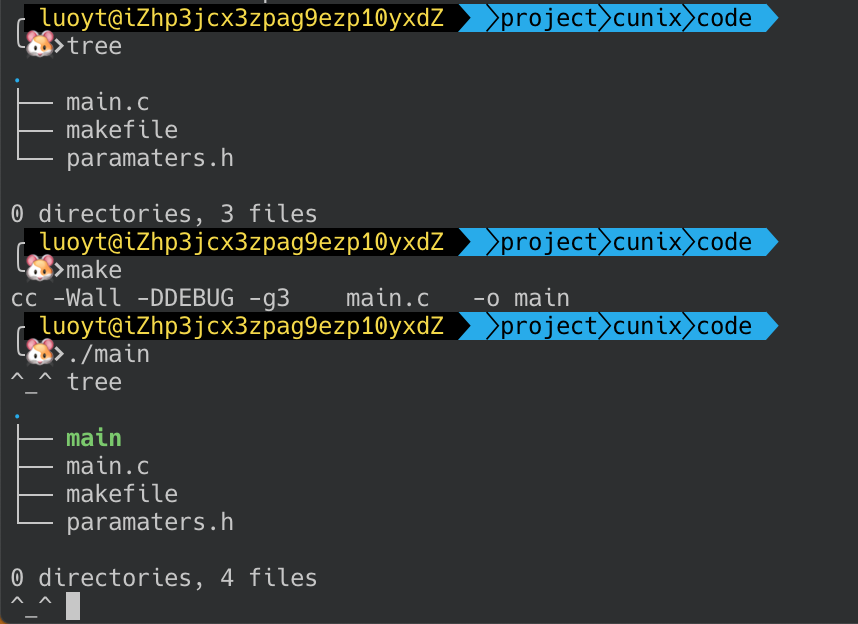
\includegraphics[width=0.7\textwidth]{images/init}
	\caption{\label{init}编译运行文件执行结果}
\end{figure}
\end{frame}

\subsection{命令执行}
\begin{frame}{正确执行简单命令}
在此我们演示几个较为简单地命令(ls, cd, cowsay等),如图\ref{base}所示:
\begin{figure}
	\centering
	\begin{minipage}[t]{0.45\textwidth}
		\centering
		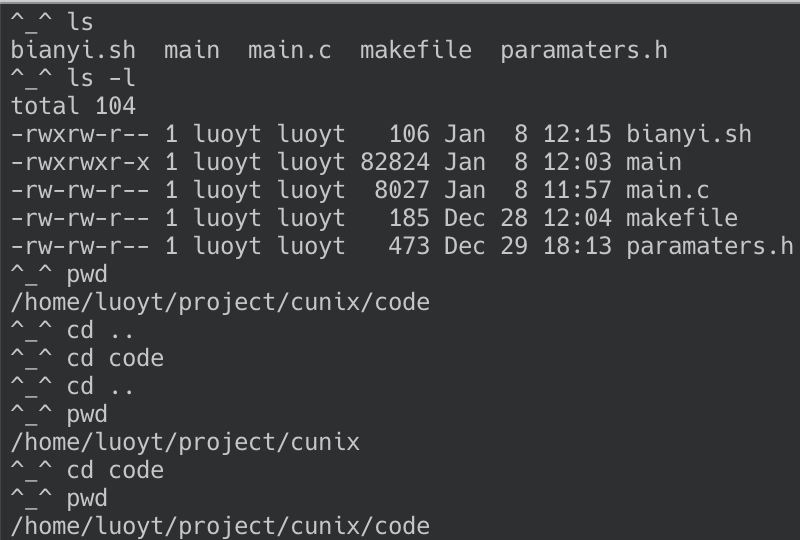
\includegraphics[width=4cm]{images/base1}
	\end{minipage}
	\begin{minipage}[t]{0.45\textwidth}
		\centering
		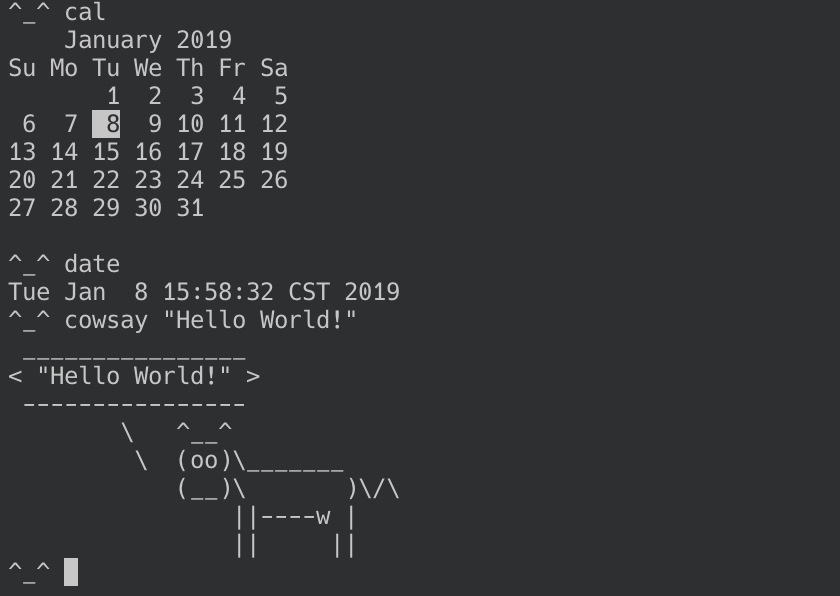
\includegraphics[width=4cm]{images/base2}
	\end{minipage}
	\caption{\label{base}简单命令执行示意图}
\end{figure}

\end{frame}

\begin{frame}{输入输出重定向到文件}
在此我们演示将命令输入重定向和输出重定向的功能,如图\ref{redirect}所示:
\begin{figure}[htbp]
	\centering
	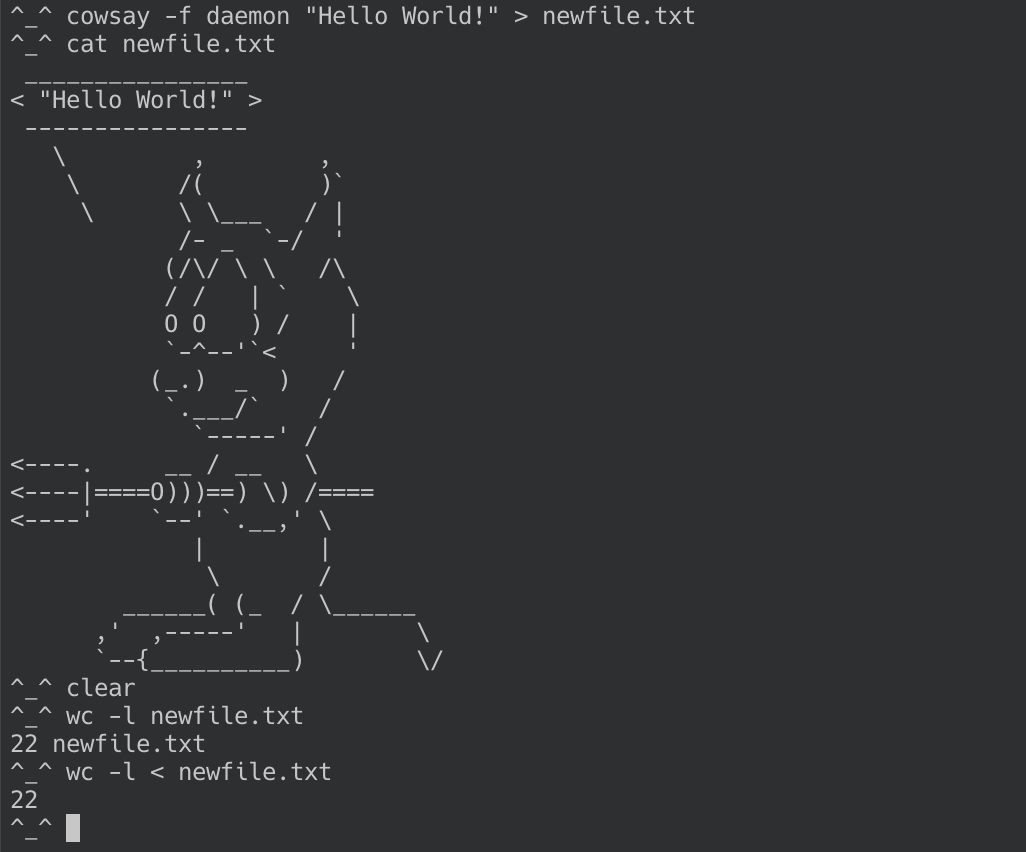
\includegraphics[width=0.65\textwidth]{images/redirect}
	\caption{\label{redirect}输入输出重定向运行结果}
\end{figure}
\end{frame}

\begin{frame}{管道操作}
在此我们通过管道操作符'|'演示管道操作,如图\ref{pipe}所示:
\begin{figure}[htbp]
	\centering
	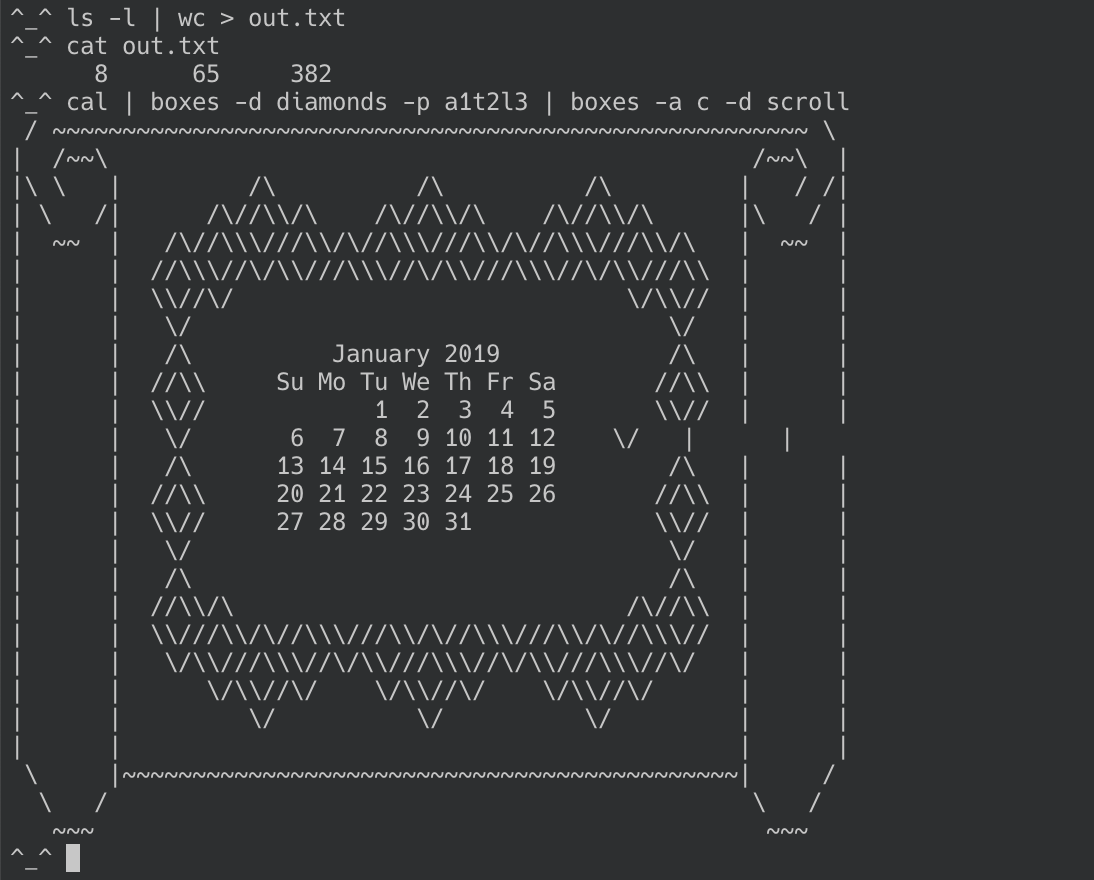
\includegraphics[width=0.65\textwidth]{images/pipe}
	\caption{\label{pipe}管道操作结果示意图}
\end{figure}
\end{frame}

\begin{frame}{后台执行程序}
在此我们对比演示'sleep 10'和'sleep 10 \&'两个命令的区别,如图所示:
\begin{figure}[htbp]
	\centering
	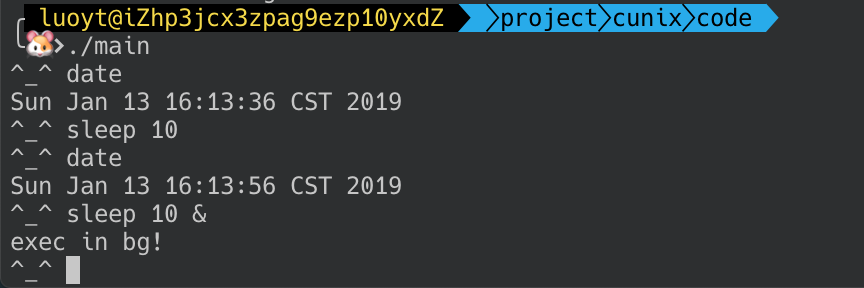
\includegraphics[width=0.95\textwidth]{images/bg}
	\caption{\label{bg}后台执行命令结果示意图}
\end{figure}
\end{frame}

\begin{frame}{历史记录操作}
在此我们演示了'history'命令的执行结果,如图\ref{history}所示:
\begin{figure}[htbp]
	\centering
	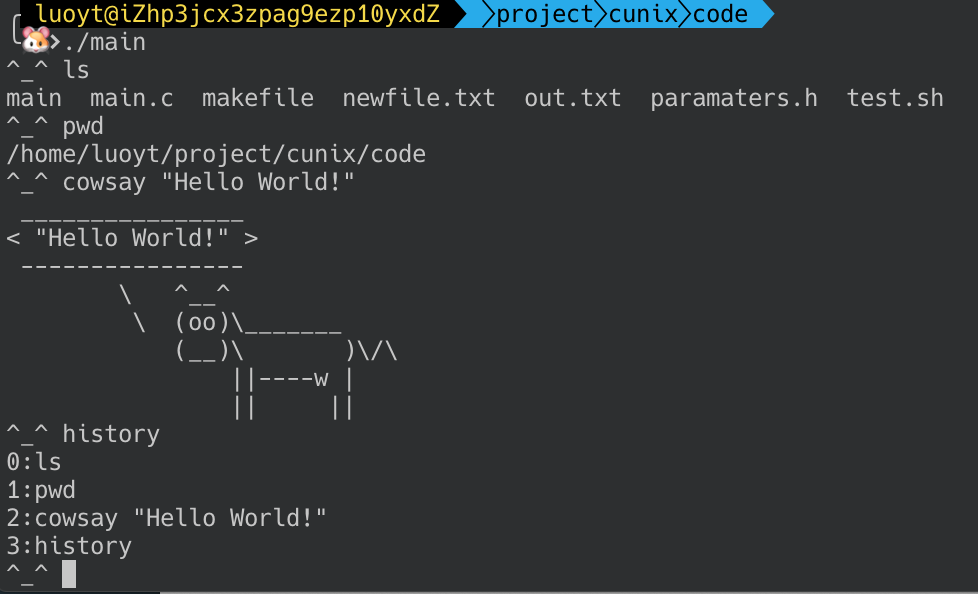
\includegraphics[width=0.95\textwidth]{images/history}
	\caption{\label{history}history结果示意图}
\end{figure}
\end{frame}
\begin{frame}{环境变量设置}
在此我们执行export设置环境变量并且用echo输出环境变量作为演示,如\ref{envvar}所示:
\begin{figure}[htbp]
	\centering
	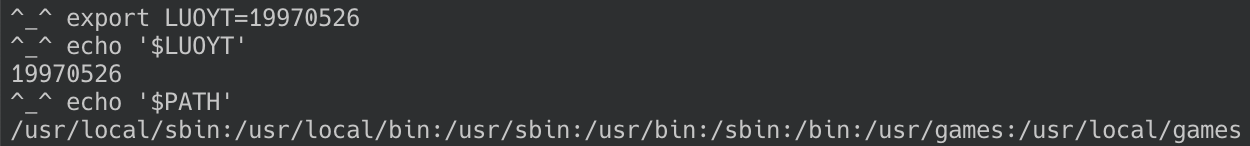
\includegraphics[width=0.95\textwidth]{images/envvar}
	\caption{\label{envvar}环境变量设置与输出示意图}
\end{figure}
\end{frame}
\begin{frame}{简单脚本执行}
在此我们首先使用vim建立一个脚本文件,然后在yaush中执行此脚本文件,如图\ref{script}所示:
\begin{figure}[htbp]
	\centering
	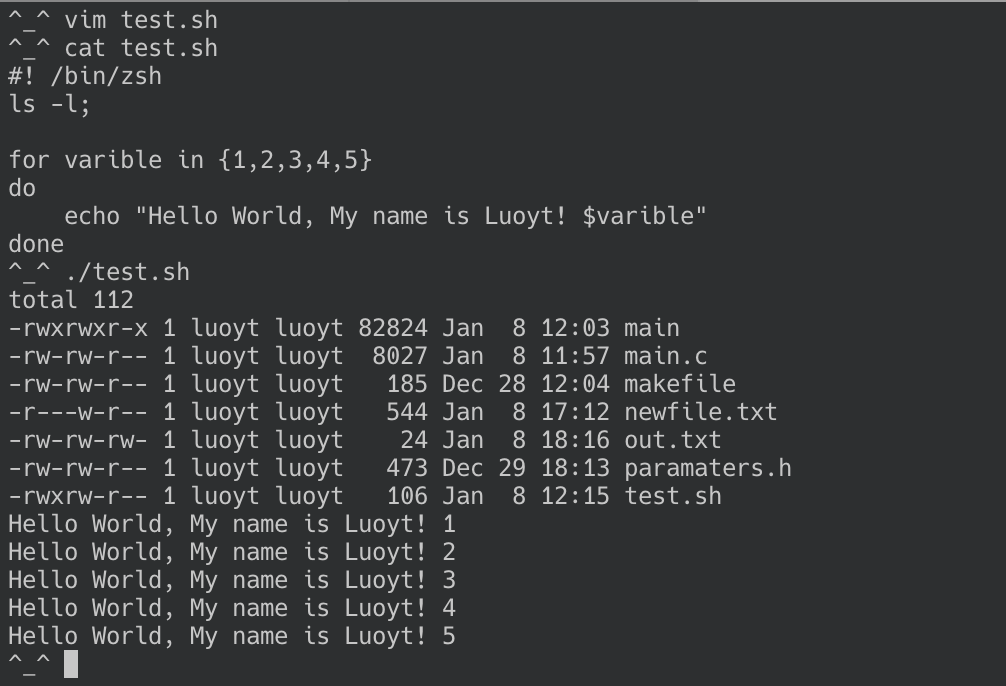
\includegraphics[width=0.75\textwidth]{images/script}
	\caption{\label{script}简单脚本执行结果示意图}
\end{figure}
\end{frame}

\section{总结}
\begin{frame}{总结}
本次大作业简单地实现了一个命令执行程序(shell),但是在使用自己shell的过程中发现和自带的bash、zsh等成熟的shell相比较还是差很多。通过本次实验,充分复习了上课学到的知识也通过自己的查阅资料学习到了很多新的东西,希望在以后能够用到自己的科研以及工作之中。但是由于考试的原因,实现的shell并不完美,希望之后有时间能够在以下几个方面进行优化。

\begin{itemize}
	\item 能够正确使用上下左右箭头进行调整;
	\item 能够支持中文;
	\item 能够实现自动补全、快捷键等。
\end{itemize}
\end{frame}

\begin{frame}{致谢}
\begin{itemize}
	\item 感谢老师一学期以来的辛勤讲述;
	\item 感谢助教一学期认真批改作业以及对作业的指导;
\end{itemize}
\end{frame}



\end{document}